\section{Энергия основного состояния}
Зная вектор вероятностей, можно вычислить среднюю энергию. Вернёмся к формулам (\ref{min_energy} - \ref{rec}) и выполним усреднение. Рассмотрим следующую функцию:
\begin{equation}
  E_n = \frac 1 2 (|h_n + H_n + J| + |h_n + H_n - J|)
\end{equation}

\begin{figure}
\centering
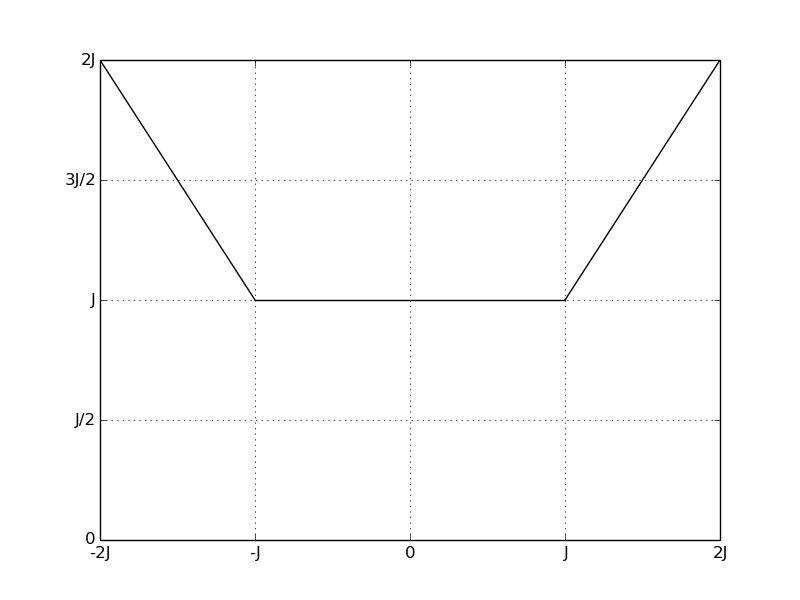
\includegraphics[width=0.9\textwidth]{figure_1.png}
\caption{Зависимость $E_n$ от $h_n+H_n$}
\end{figure}

Энергия основного состояния тогда:
\begin{equation}
  E = \left< E_n \right>
\end{equation}
Заметим, что состояния, для которых $|H_n + h_n| < J$, вносят вклад $J$ в энергию. Вычислим вероятность состояний, которые дают нетривиальный вклад:
\begin{align}
	\begin{split}
   &P(H_n + h_n = J+h) = P(H_n=J \text{ и } h_n = h) = p_3 b_0\\
   &P(H_n + h_n = J + J \text{mod} h) = P(H_n=-J+kh \text { и } h_n =h)=p_3 a_k\\
   &P(H_n + h_n = -J-h) = P(H_n=-J \text{ и } h_n = -h) = p_1 a_0\\
   &P(H_n + h_n =- J - J \text{mod} h) = P(H_n=J-kh \text{ и } h_n =-h)=p_1 b_k\\
   \end{split}
\end{align}

Подставляя выражения для $a_0, b_0, a_k, b_k$ через $x^{k+1}_i$ и $x^{k}_i$, получим искомую энергию:
\begin{equation}
		E = J + h p_3 x^{k+1}_{k+1}  + h p_1 x^{k+1}_0 + (J \text{mod} h) (p_3 (x^k_k - x^{k+1}_{k+1}) +p_1(x^k_0-x^{k+1}_0))
\end{equation}

Заметим, что энергия есть кусочно-непрерывная функция шага внешнего поля $h$. Полученный результат согласуется с известным точным решением \cite{hamasaki2004exact}, но не использует предел нулевой температуры.



\newpage